\documentclass[12pt,a4papper]{article}
\usepackage[letterpaper,margin=0.75in]{geometry}
\usepackage[utf8]{inputenc}
\usepackage[brazil]{babel}
\usepackage{mdwlist}
\usepackage[table,xcdraw]{xcolor}
\usepackage[T1]{fontenc}
\usepackage{textcomp}
\usepackage{tgpagella}
% \pagestyle{empty}
\pagenumbering{arabic}
\setlength{\tabcolsep}{0.5em}

\usepackage{authblk}

\title{Modelo matemático para o crescimento da COVID-19 em estados brasileiros}
% \author[1]{Daniel Girardi}
% \author[1]{Marcelo D'allangol}
% \author[2]{Nilton da Silva Branco}
% \affil[1]{Departamento de Ciências Exatas e Educação - Universidade Federal de Santa Catarina}
% \affil[2]{Departamento de Física - Universidade Federal de Santa Catarina}
\author{Daniel Girardi$^{1}$, Marcelo Alloy D'allangol$^{1}$ e Nilton da Silva Branco $^{2}$  \\
        \small $^{1}$Departamento de Ciências Exatas e Educação - Universidade Federal de Santa Catarina \\
        \small $^{2}$Departamento de Física - Universidade Federal de Santa Catarina \\
}
% \date{} % Comment this line to show today's date

% \date{Abril de 2020}

\usepackage{natbib}
\usepackage{graphicx}

\begin{document}

\maketitle

\begin{abstract}
Lorem ipsum dolor sit amet, consectetur adipiscing elit. Vestibulum pretium libero non odio tincidunt semper. Vivamus sollicitudin egestas mattis. Sed vitae risus vel ex tincidunt molestie nec vel leo. Vestibulum ante ipsum primis in faucibus orci luctus et ultrices posuere cubilia Curae; Maecenas quis massa tincidunt, faucibus magna non, fringilla sapien. In ullamcorper justo a scelerisque egestas. Ut maximus, elit a rutrum viverra, lectus sapien varius est, vel tempor neque mi et augue. Fusce ornare venenatis nunc nec feugiat. Proin a enim mauris. Mauris dignissim vulputate erat, vitae cursus risus elementum at. Cras luctus pharetra congue. Aliquam id est dictum, finibus ligula sed, tempus arcu. 
\end{abstract} \hspace{10pt}

\section{Introdução}


Dia 11 de março de 2020, em uma coletiva de imprensa, o Diretor Geral da Organização Mundial da Saúde (OMS) declarou que a COVID-19 já era caracterizada como uma pandemia \cite{WHOpandemic}. A declaração motivou o início da ação contra a doença em diversos países. Em artigo publicado em 30 de março no \textit{The Lancet}, Richard Verity do Imperial College, estimou que a taxa de mortalidade da COVID-19 é próxima de $1,38\pm 0,15$ com uma confiança de $95\%$ em seu resultado \cite{verity2020estimates}. Apesar de  menores que a SARS \cite{wang2004simulating} e a MERS \cite{majumder2014estimation} essa taxa é um pouco maior que o dobro da taxa da H1N1. Cabe ressaltar a importância histórica que a Inglaterra possui no estudo das taxas de mortalidade \cite{robertson1996reckoning}. 

O resultado obtido por Verity, possui grande discrepância do observado para os dados globais. Na tabela \ref{tab:mortality}, apresenta-se as taxas de mortalidade em 03 de abril de 2020 para os países com o maior número de casos, além do Brasil e o valor Mundial. O único país que apresenta taxa de mortalidade próxima da estimada é a Alemanha. Pode-se atribuir 5 fatores para essas discrepâncias:
\begin{enumerate}
    \item \textbf{Subnotificação}: Uma parcela da população manifesta a doença na forma leve, não necessitando de auxílio médico. Portanto, não há como ter o verdadeiro número de casos, apenas estimativas. Além disso, com o aumento exponencial do número de casos, os laboratórios não possuem condições de testar todos os casos suspeitos.
    \item \textbf{Distribuição de idades na população}: A Itália, por exemplo, possui uma população de idosos muito maior que a população dos outros países. Os dados mostram que a mortalidade da COVID-19 é afetada pela idade e comorbidades dos infectados \cite{wu2020characteristics};
    \item \textbf{Densidade populacional}: Os grandes centros são os mais afetados. Primeiro, por receberem muitas pessoas de fora, mas também por apresentarem maior densidade populacional. O aumento da densidade populacional dificulta o isolamento social e propicia a mobilidade do vírus.
    \item \textbf{Estrutura do sistema de saúde}: O maior problema é a sobrecarga no sistema de saúde e a falta de estrutura para tratar todos os infectados. A Itália está próxima do colapso do sistema de saúde \cite{armocida2020italian} e há mais de uma semana que idosos não tem sido atendidos para que possam atender pessoas com maior perspectiva de sobrevivência.
    \item \textbf{Qualificação do profissional da saúde}: A sobrecarga no sistema de saúde também afeta a qualidade do sistema de saúde. As equipes médicas estão sendo reduzidas devido a contaminação dos profissionais que fazem o atendimento aos infectados. Para suprir a mão de obra afastada, profissionais de diferentes setores tem sido realocados para as Unidades de Terapia Intensiva. Em muitos casos, esses profissionais não possuem a qualificação atuar com pacientes críticos. No Brasil, os profissionais da área da saúde estão sendo convocados para cadastramento e treinamento obrigatório \cite{chamamentoMS}.
\end{enumerate}{}

\begin{table}[h]
\centering
\caption{\centering Taxa de mortalidade para os países com maior número de casos e o Brasil. }
\label{tab:mortality}
\begin{tabular}{|c|c|c|c|c|c|c|}
\hline
\textbf{País}   & \textbf{Casos} & \textbf{Mortes} & \textbf{Mortalidade} & \textbf{\begin{tabular}[c]{@{}c@{}}Casos\\ por 1M Hab.\end{tabular}} & \textbf{\begin{tabular}[c]{@{}c@{}}Mortes\\ por 1M Hab.\end{tabular}} & \textbf{\begin{tabular}[c]{@{}c@{}}Mortalidade\\ por 1M Hab.\end{tabular}} \\ \hline
EUA      & 245442   & 6098   & 2,48\%  & 742   & 18   & 2,43\%  \\ \hline
Itália    & 115242   & 13915  & 12,07\% & 1906  & 230  & 12,07\% \\ \hline
Espanha    & 11771    & 10935  & 92,90\% & 2518 & 234  & 9,29\%                                                                     \\ \hline
Alemanha         & 86667          & 1129            & 1,30\%               & 1034                                                                 & 13                                                                    & 1,26\%                                                                     \\ \hline
França          & 59105          & 5387            & 9,11\%               & 905                                                                  & 83                                                                    & 9,17\%                                                                     \\ \hline
Reino Unido              & 38168          & 3605            & 9,45\%               & 562                                                                  & 53                                                                    & 9,43\%                                                                     \\ \hline
\rowcolor[HTML]{FFFE65} 
\textbf{Brasil} & \textbf{8076}  & \textbf{329}    & \textbf{4,07\%}      & \textbf{38}                                                          & \textbf{2}                                                            & \textbf{5,26\%}                                                            \\ \hline
\rowcolor[HTML]{C0C0C0} 
Mundial           & 1039922        & 55170           & 5,31\%               & 133,4                                                                & 7,1                                                                   & 5,32\%                                                                     \\ \hline
\end{tabular}
\centring Fonte: WorldMetrics \cite{worldmetrics}.
\end{table}

O que os dados sugerem é que fazer uma análise geral para um país tão grande quanto o Brasil será um erro. O Brasil tem $80\%$ da área da Europa, somos um país continental e com muitas diferenças entre estados na mesma região. Qualquer proposta de modelo de previsão, precisa ser trabalhada localmente, idealmente deveria ser analisado cada município ou microrregião de cada estado. Contudo, o esforço seria imenso e não há como uma única equipe cobrir o trabalho para todos os municípios ou microrregiões brasileiras. 

Nas próximas seções apresenta-se primeiro as demandas para um sistema preditivo, o modelo matemático proposto, nosso objetivo de implementação e os resultados esperados. Ao final, apresentamos as demandas para execução deste projeto.

\section{Perguntas do problema}

A primeira proposta para o combate a pandemia é o isolamento social. Por isso, a maioria dos países e estados brasileiros entraram num regime de quarentena coletiva. O comércio não essencial está fechado na maioria das cidades brasileiras e com isso começa a pressão de diversos setores econômicos pelo fim da quarentena. Assim, surgem as primeiras questões: \textbf{Por quanto tempo precisaremos ficar em quarentena? Qual o plano de retorno das atividades comerciais não essenciais?} É importante responder essas perguntas, não é possível negligenciar totalmente a importância da atividade econômica. Contudo, não se pode colocar em risco a vida das pessoas, sob o risco de impactar a economia, de forma mais agressiva que o isolamento.

A segunda forma de combate é o tratamento médico dos infectados. Em muitos estados brasileiros, o Sistema Único de Saúde (SUS) já estava operando perto do limite de atendimento. Com o estouro da pandemia e o aumento exponencial da demanda por leitos nos hospitais, vemos estados criando hospitais de campanha. Estruturas provisórias que visam ampliar a capacidade hospitalar para atender esse aumento na demanda. Dessa forma, mais perguntas surgem: \textbf{Como o nosso sistema de saúde será impactado pela pandemia? Quantos leitos precisam ser criados para atender a demanda? Qual o impacto, na contenção da pandemia, novos leitos provocam?}

A última pergunta é: \textbf{Ao fim da quarentena, a doença não vai voltar a crescer?} Existem outras perguntas, mas este modelo se propõe a fornecer respostas e indícios para essas perguntas.


\section{Modelo matemático}

Propõe-se um modelo matemático determinístico baseado em 10 compartimentos.  Cada compartimento, corresponde a uma classe de indivíduo dentro do ciclo da epidemia. Os compartimentos são: 
\begin{enumerate}
    \item Saudáveis (S): pessoas que podem ser contaminadas;
    \item Expostos (E): pessoas que já foram contaminadas, mas ainda estão no período de incubação do vírus. Ou seja, não manifestam sintomas e nem contaminam indivíduos saudáveis;
    \item Infectados (I): pessoas que estão infectando outras pessoas. Neste compartimento, estão todos que são capazes de infectar outras pessoas, independente de estarem confirmados ou não para a COVID-19;
    \item Infectados Graves ($I_G$): pessoas infectadas que evoluíram para o estado grave da doença e que precisam de auxílio médico;
    \item Hospitalizados em leito comum ($H_L$): As pessoas que buscaram ajuda em hospitais e foram admitidas para internação;
    \item Hospitalizados em UTI ($H_u$): pessoas em estágio mais grave da doença e que demandam de suporte de ventilação mecânica;
    \item Hospitalizados em leito comum com ventilação mecânica ($H_{lv}$): pessoas que deveriam estar em uma UTI, mas por falta de leito em UTI, são colocadas em leitos comuns e com ventilação mecânica (quando há ventiladores disponíveis);
    \item Hospitalizados em leito comum em estado grave ($H_{lg}$): pessoas que deveriam estar em uma UTI, mas com a falta de UTI e ventilador mecânico para os leitos comuns, estão num leito comum mas em estado grave;
    \item Curados (C): pessoas que se curaram da COVID-19. A priori, essas pessoas são consideradas imunes e, portanto, não podem mais ser reinfectadas;
    \item Mortos (M): pessoas que morreram em decorrência da COVID-19.
\end{enumerate}

A modelagem é feita para lidar com valores absolutos. Ou seja, as simulações são feitas utilizando o tamanho real da população, número total de leitos e leitos de UTI disponíveis para a região simulada. Essa abordagem visa gerar mais transparência para os gestores. A seguir, apresenta-se o modelo matemático para cada compartimento e como os compartimentos estão interligados.

\subsection{Saudáveis (S)}
A fração $\delta$ de \textit{Saudáveis} representa a parcela da população que não está seguindo as normas de quarentena ou se expondo ao vírus. Isso inclui o percentual de pessoas que tenta seguir a regra da quarentena mas precisa sair de casa para comprar mantimentos. Estes, podem ser contaminados pelos \textit{Infectados} (I) e \textit{Infectados Graves} ($I_g$). A taxa de contágio de cada um desses indivíduos é dada por $\alpha=\frac{R0}{N.T_{infec}}$, onde $R0$ é o número de pessoas que cada pessoa infectada contamina \cite{liu2020reproductive}, N é o número de pessoas na população e $T_{infec}$ é o número médio, em dias, que uma pessoa fica infectada. A parcela da população infectada torna-se \textit{Exposta} (ver figura \ref{covidS}). 
\begin{equation}
	\frac{dS}{dt}= -S\delta(\alpha_i I +\alpha_{ig}I_g)
\end{equation}
\begin{figure}[!h]
\label{covidS}
	\centering
	\includegraphics[scale=0.4]{covidS}
	\caption{Diagrama da equação dos Saudáveis.}
	\label{fig:universe}
\end{figure}

\subsection{Expostos (E)}
Os \textit{Expostos} aumentam conforme há a contaminação dos \textit{Saudáveis} e com o tempo evoluem a uma taxa $\beta=\frac{1}{T_{inc}}$, onde $T_{inc}$ é o período médio, em dias, que uma pessoa leva para manifestar a doença após ser infectada.  A evolução desse estado é a ida para o estado \textit{Infectado}.

\begin{equation}
	\frac{dE}{dt}= S(\alpha_i I +\alpha_{ig}I_g) - \beta E
\end{equation}
\begin{figure}[!h]
	\centering
	\includegraphics[scale=0.4]{covidE}
	\caption{Diagrama da equação dos Expostos.}
	\label{fig:universe}
\end{figure}

\subsection{Infectados (I)}
Esses são os que eram \textit{Expostos}, mas evoluíram para o estado ativo da doença. \textbf{Por definição}, estes são os indivíduos que podem contaminar indivíduos saudáveis. Importante ressaltar que nesse modelo, não fazemos distinção entre testados e não testados, ambos são considerados infectados. Estes podem evoluir a uma taxa $\lambda_I=\frac{1}{T_{infec}}$ para curados ou evoluir a uma taxa $\zeta$ para \textit{Infectados no estado Grave}.
\begin{equation}
	\frac{dI}{dt}= \beta E -\lambda_i I - \zeta I
\end{equation}
\begin{figure}[!h]
	\centering
	\includegraphics[scale=0.4]{covidI}
	\caption{Diagrama da equação dos Infectados.}
	\label{fig:universe}
\end{figure}

\subsection{Infectados Graves ($I_G$)}
São os que manifestaram o quadro grave e que necessitam de internação hospitalar. Contudo, os hospitais possuem uma capacidade de leitos de internação que são definidos pelo número de leitos comuns ($\kappa_L$) mais o número de leitos de UTI ($\kappa_U$). Portanto, uma parcela $\gamma$ destes, irão procurar os hospitais mas só serão recebidos de acordo com a disponibilidade de leitos $(1-\frac{H_l+H_u+H_{lg}+H_{lv}}{\kappa_l+\kappa_u})$. Se a soma te todos os hospitalizados  $H_l+H_u+H_{lv}+H_{lg}$ (leito comum, UTI, leito comum com ventilação mecânica e leito comum em estado grave) for igual a capacidade total dos hospitais $\kappa_l+\kappa_u$, então esse indivíduo continuará no estado $I_G$, ou seja, ele não foi acolhido por nenhum hospital. Neste estado, os indivíduos morrem a uma taxa $\mu_{ig}$ e se curam a uma taxa $\lambda_{ig}$. 

\begin{equation}
	\frac{dI_G}{dt}= \zeta I -(1-\frac{H_l+H_u+H_{lg}+H_{lv}}{\kappa_l+\kappa_u})\gamma I_G - \lambda_{ig} I_G - \mu_{ig} I_G
\end{equation}
\begin{figure}[!h]
	\centering
	\includegraphics[scale=0.4]{covidIg}
	\caption{Diagrama da equação dos Infectados Graves.}
	\label{fig:universe}
\end{figure}
\subsection{Hospitalizados em Leito Comum ($H_l$)}
Uma vez hospitalizado, o indivíduo vai para um leito comum e dentro do hospital ele pode seguir alguns caminhos a depender da evolução da doença. Alguns pacientes se curam a uma taxa $\lambda_{hl}$. Outros pacientes irão evoluir para um estado grave, necessitando da internação em UTI, com uma taxa de agravamento igual a $\nu_u$. Além disso, todos os pacientes em estado mais graves não se curam automaticamente. Antes de saírem do hospital, esses pacientes retornam para o leito comum. Assim, o número de hospitalizados em leito comum, recebe os indivíduos que estavam hospitalizados em nível mais graves a taxas $\lambda$.
\begin{equation}
	\frac{dH_l}{dt}=(1-\frac{H_l+H_u+H_{lg}}{\kappa_l+\kappa_u})\gamma I_g - \lambda_{hl} H_l - \nu_uH_l + \lambda_{hu}H_u +\lambda_{lg}H_{lg} +\lambda_{lv}H_{lv}
\end{equation}
\begin{figure}[!h]
	\centering
	\includegraphics[scale=0.3]{covidHl}
	\caption{Diagrama da equação dos Hospitalizados em Leito Comum.}
	\label{fig:universe}
\end{figure}

\subsection{Hospitalizados em Leito de UTI ($H_u$)}
Os leitos de UTI são para aqueles que estiveram em leito comum, mas houve o agravamento da situação. Contudo, apenas uma fração desses pacientes podem ser recebidos pela UTI. Essa fração é definida pela capacidade de leitos na UTI $\kappa_u$. Não havendo leitos na UTI, estes são compartimentalizados em outra situação, leitos comuns com ventilador mecânico ($H_{lv}$) ou apenas leitos comuns com pacientes em estado grave ($H_{lg}$). Além disso, o indivíduo pode melhorar, voltando ao leito comum, com taxa $\lambda_{hu}$ ou morrer com taxa $\mu_{hu}$.
\begin{equation}
	\frac{dH_u}{dt}=\nu_u H_l(1 - \frac{H_u}{\kappa_{u}}) -\lambda_{hu} H_u -\mu_{hu} H_u
\end{equation}
\begin{figure}[!h]
	\centering
	\includegraphics[scale=0.4]{covidHu}
	\caption{Diagrama da equação dos Hospitalizados em Estado Grave.}
	\label{fig:universe}
\end{figure}


\subsection{Hospitalizados em Leito comum com Ventilador Mecânico ($H_{lv}$)}
Aqueles que tinham que ir para a UTI, mas não conseguiram por falta de leitos, irão para os leitos que possuírem ventiladores mecânicos, até a capacidade de ventiladores mecânicos disponíveis, além dos da UTI, definida pelo valor $\kappa_v$. O termo para essa taxa é: $\nu_u H_l \frac{H_u}{\kappa_{u}}(1-\frac{H_{lv}}{\kappa_{v}})$. Além disso, os indivíduos nessa situação melhoram a uma taxa $\lambda_{lv}$, retornando para o compartimento $H_l$ (leito comum) e morrem a taxas $\mu_{lv}$.

\begin{equation}
	\frac{dH_{lv}}{dt}=\nu_u H_l\frac{H_u}{\kappa_{u}}(1-\frac{H_{lv}}{\kappa_{v}})  - \lambda_{lv}H_{lv}-\mu_{lv}H_{lv}
\end{equation}
\subsection{Hospitalizados em Leito comum em estado grave ($H_{lg}$)}
Os que não conseguirem ventilador mecânico no leito, ficam em estado grave em um leito comum. Não há necessidade de definir uma capacidade de leitos pois o indivíduo nesse estado já tiveram seu leito contabilizados na admissão ao hospital. Além disso, melhoram com uma taxa $\lambda_{lg}$ e morrem a taxa $\mu_{lg}$.

\begin{equation}
	\frac{dH_{lg}}{dt}=\nu_u H_l\frac{H_{lv}}{\kappa_{v}}\frac{H_u}{\kappa_{u}} -\lambda_{lg}H_{lg}-\mu_{lg}H_{lg} 
\end{equation}

\subsection{Mortos (M) e Curados (C)}
Neste modelo, só morrem aqueles que estão em Infectados Graves e os que estão nos hospitais em estados mais graves. Atribuímos que aqueles que estão em leito comum, não morrem. Precisam agravar o caso antes de morrer.

\begin{equation}
	\frac{dM}{dt}=\mu_{ig}I_{g} + \mu_{hu}H_u +\mu_{lv} H_{lv}+\mu_{lg} H_{lg}
\end{equation}

Os curados são aqueles que se recuperaram da doença e, enquanto não houver dados contrários, não podem mais ser reinfectados pelo vírus.
\begin{equation}
	\frac{dC}{dt}=\lambda_i I + \lambda_{ig} I_g +\lambda_{hl}H_l 
\end{equation}

\begin{figure}[!h]
\label{covid}
	\centering
	\includegraphics[scale=0.4]{covid}
	\caption{Visão geral dos caminhos para a COVID-19}
	\label{fig:universe}
\end{figure}




\section{Resultados esperados}

A proposta é que esse modelo seja implementado como uma página na Internet capaz de fazer a simulação no navegador. Essa página teria informações públicas, oriundas das análises das simulações e informações privadas compartilhada entre os usuários credenciados. O objetivo desse modelo é poder fazer a análise da evolução e previsões de forma distribuída. Cada estado ou microrregião, teria uma pessoa responsável por alimentar o sistema de simulação com os dados da sua região. Estando todas esses dados e simulações concentrados em um único local, é mais fácil analisar o impacto nacional das ações. Inclusive com a possibilidade de fazer simulações levando em conta a mobilidade dos indivíduos entre as regiões.

As únicas variáveis deste modelo que podem ser controladas pelas políticas públicas são: $\kappa_u$, $\kappa_l$ e $\kappa_v$ que são as capacidades de leitos de UTI, leitos comum e ventiladores mecânicos (além dos que estão nos leitos de UTI). Ao analisar o impacto que a mudança dessas variáveis causam na dinâmica da epidemia, pode-se guiar a ação do poder público. Essa análise pode inclusive ser guiada por fatores econômicos como custo de implementação de novos leitos \textit{versus} prevalência\footnote{Prevalência se refere ao número de casos de uma doença num determinado intervalo de tempo.} da COVID-19.

Outra variável, parcialmente controlável, é o $\delta$. Ela remete diretamente as medidas de contenção e de isolamento social. A proposta é avaliar cenários em que o $\delta$ possa ir sendo aumentado. Por exemplo, conjecturando que hoje temos $70\%$ de pessoas em quarentena ($\delta=30\%$). Qual o impacto para a prevalência da COVID-19 se a cada semana as medidas de isolamento social sejam relaxadas em $10\%$? Assim, é possível estimar as consequências das políticas públicas propostas para o fim quarentena, de forma a garantir a segurança da população, sem comprometer o sistema de saúde e provocar o menor impacto possível na economia. 


\section{Demandas para execução do projeto}

No momento, está sendo desenvolvido uma Prova de Conceito (PdC) desta proposta de realizar essa modelagem online. Essa PdC vai servir para fazermos uma análise piloto para o estado de SC e pode ser repassada para que os outros estados utilizem esse mesmo modelo e sistema de simulação. Para o sucesso dessa análise piloto, precisamos dos dados oriundos da secretaria de saúde. 

Para alcançarmos o objetivo de criar uma plataforma online onde cada estado ou microrregião possa fazer a sua análise, vamos precisar de uma equipe técnica para desenvolver o sistema que salve os dados inseridos, gerencie o acesso e as credenciais de acesso, permita o compartilhamento dos dados e a curadoria do que será publicado para a comunidade em geral. Os proponentes do projeto não tem a habilidade para o desenvolvimento de tal plataforma. Caberia ao poder público buscar parceiros ao projeto para este desenvolvimento.



	
% https://ciis.fmrp.usp.br/covid19/epcalc/public/index.html
	
% \section{Conclusion}
	
\bibliographystyle{unsrt}
\bibliography{references}
\end{document}
